\chapter{Metodologia}

\section{Problem modeling}
\subsection{General model}
\subsection{Symmetric attenuation}
\subsection{Weak-source regime}
\clearpage
\section{Preprocesamiento}
\subsection{Filtering}
\subsubsection{Filter desing}
\subsection{Normalization}
\subsection{Whitening}
\section{Independent Component Analysis (ICA)}

Independent Component Analysis (ICA) is a fundamental processing technique within Blind Source Separation aimed at recovering latent source signals from observed mixtures without any prior knowledge of the sources or mixing process. As mentioned in previous sections, EMG signals may benefit from this power tool as it allows to decompose multichanel recordings into meaningful physiological components, potentially corresponding to muscle and neural sources.

From a signal processing perspective, ICA a

This section introduces the mathematical formulation and derivation of ICA as well as its basic assumptions and principles. Additionally, a widely used implementation (FastICA) is described, followed by a discussion of ICA's challenges and limitations.
\subsection{Problem formulation}
ICA is originally formulated for linear and instananeous mixing models. Let $s(t)=[s_1(t),...,s_n(t)]$ be an array of source signals and $x(t)=[x_1(t),...,x_n(t)]$ the recorded mixtures. The relationship between both is then given by:

\begin{equation}
    x(t)=As(t)+n(t)
\end{equation}

\noindent where $\mathbf{A}$ is an unknown mixing matrix and  $\mathbf{n}(t)$ represents additive noise.

Considering the given the case, the objective of ICA is to estimate a separating matrix $\mathbf{W}$ such that:

\begin{equation}
    \hat{\mathbf{s}}(t) = \mathbf{W} \mathbf{x}(t)
\end{equation}

\noindent recovers the original sources with no prior information. 

However, the recovery of the sources is subject to inherent ambiguities. In particular, ICA cannot determine the original scaling or ordering of the sources. This is due to the fact that any scaling or permutation applied to the sources can be compensated by the mixing matrix without affecting the observed signals. As a result, the estimated sources can be expressed as:

\begin{equation}
    \hat{\mathbf{s}}(t) = \mathbf{P} \mathbf{D} \mathbf{s}(t)
\end{equation}

\noindent where $\mathbf{P}$ is a permutation matrix and $\mathbf{D}$ is a diagonal scaling matrix. These ambiguities are inherent to the ICA algorithm and, for that reason, the original order and amplitude of the sources cannot be uniquely determined by the observed mixtures.


\subsection{Assumptions of ICA}

The ICA framework relies on a set of assumptions that ensure the identifiability of the source signals from the observed mixtures. These assumptions are fundamental to the correct operation of the algorithm and must be considered when applying ICA to real-world signals such as EMG.

\begin{itemize}

\item \textbf{Statistical independence} $\rightarrow p(s_1,s_2)=p(s_1)p(s_2)$ \\ \\
The source signals $s_i(t)$ are assumed to be mutually independent. This is the key assumption of ICA, as the separation is achieved by maximizing statistical independence between the estimated components.

\item \textbf{Non-Gaussianity} \\

\underline{At most one source is allowed to follow a Gaussian distribution}. ICA exploits higher-order statistics (such as kurtosis or negentropy) to separate signals, and therefore relies on the non-Gaussian nature of the sources.

\item \textbf{Linear instantaneous mixing} \\

The observed signals are assumed to be linear combinations of the sources \underline{without temporal delays}. If this was not ture, there could not be any static matrix $\mathbf{A}$ that represents the mixing.

\item \textbf{Full-rank mixing matrix} \\

The mixing matrix $\mathbf{A}$ must be invertible. This ensures that the sources can potentially be recovered from the mixtures.

\item \textbf{Number of observations}
$\rightarrow n_{mixtures} \geq n_{sources}$\\

The number of observed mixtures must be greater than or equal to the number of sources, allowing the separation problem to be well-posed.

\end{itemize}

In practice, these assumptions are only approximately satisfied, particularly in biomedical applications such as EMG signal processing. For example, sources may show partial statistical dependence, the mixing process may include delays and measurements are typically affected by noise. These non-idealities from real world applications can significantly impact the performance of ICA-based methods.

\subsection{ICA derivation (2D)}
To gain further understanding of the ICA process, a geometric and mathematical derivation is presented in the two-dimensional case, which corresponds to the specific model analyzed in this work.

Let $\begin{pmatrix}
x_1(t)  \\
x_2(t)
\end{pmatrix}= 
\overbrace{
\begin{pmatrix}
a_{11} & a_{12} \\
a_{21} & a_{22}
\end{pmatrix}
}^{\mathbf{A}}
\begin{pmatrix}
s_1(t)  \\
s_2(t)
\end{pmatrix}
$, where $x_1(t)$ and $x_2(t)$ are coordinates of $X(t)$ in $\mathbb{R}^2$. Since we do not know the values of $a_{i,j}$ the problem cannot be solved by simply calculating $W=A^{-1}$. Instead, the proposed objective is to find a series of transformations that recover a new coordinate system in which components are statistically independent. For this reason, the mixing matrix $\mathbf{A}$ can be interpreted through its singular value decomposition (SVD)\footnote{SVD factorizes a matrix as $\mathbf{A} = \mathbf{U} \mathbf{\Sigma} \mathbf{V}^T$, separating rotation and scaling components.}:

\begin{equation}
    \mathbf{A} = \mathbf{U} \mathbf{\Sigma} \mathbf{V}^T
\end{equation}

\noindent where $\mathbf{V}^T$ represents a rotation of the source signals, $\mathbf{\Sigma}$ applies a scaling along the principal directions, and $\mathbf{U}$ corresponds to a final rotation in the observation space.

Given the current decomposition, it is possible to estimate the separating matrix $W=A^{-1}=V\Sigma^{-1}U^{T}$ \footnote{Recall that rotation the inverse of rotation matrices correspond to t} which can be statistically estimated from the mixtures signals. 

Given this decomposition it is trivial to express $\mathbf{W}$
\begin{figure}[H]
    \centering
    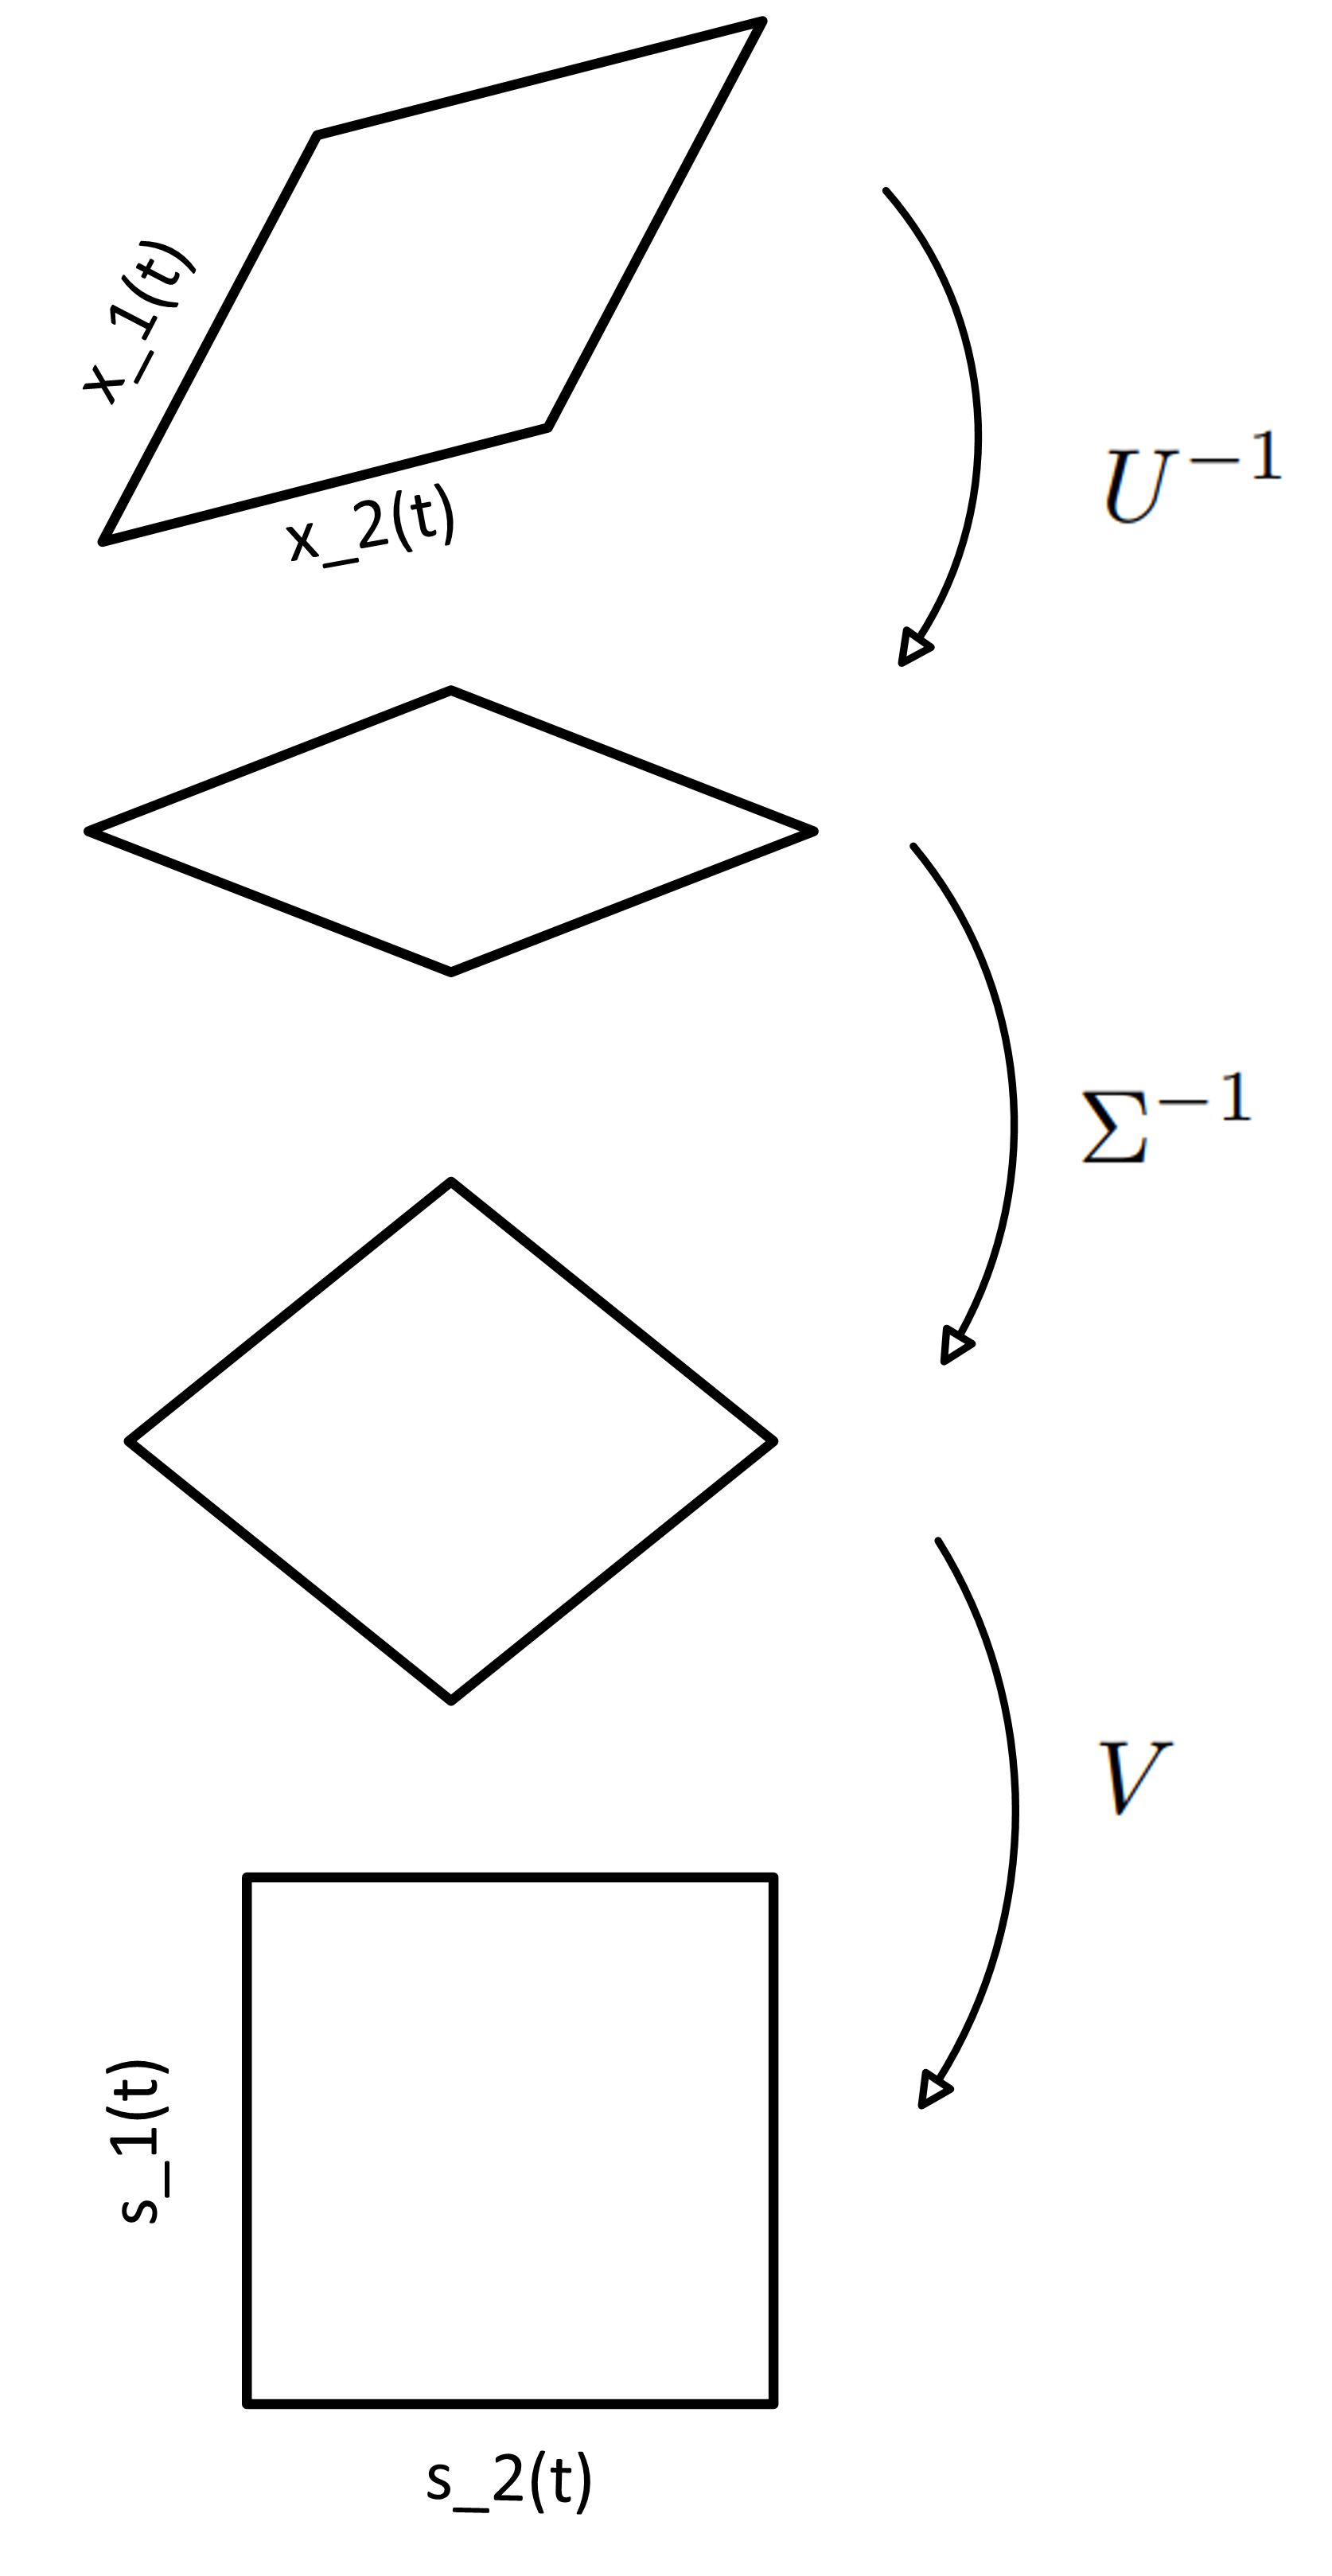
\includegraphics[height=6.5cm, width=0.35\textwidth]{figuras/ICA_geometry.png}
    \caption{Geometric interpretation of ICA in the 2D case. The observed mixtures are decorrelated with PCA (first step) and normalized (second step). Once the data is whitened the final step corresponds to the rotation that best recovers the statistically independent sources. Figure was created using the Microsof Visio tool.} 
    \label{fig:ica_geometry}
\end{figure}

\subsection{Implementations: FastICA}

Though the ICA process is straight forward, the final transformation matrix may be computationally expensive to find, given that it requires maximizing kurtosis. 

\subsection{Weak-source and noise}
Even tough ICA's process may seem 

\section{Second-Order Blind Identification (SOBI)}
\section{Constrained(ICA)}
\subsection{Possible constraints}
\subsection{Implementation}
\subsection{Avantages and limitations}
\section{Convolutive / Frequency-domain ICA}
\section{Framework}
\section{Implementacion en vivo}